% Options for packages loaded elsewhere
\PassOptionsToPackage{unicode}{hyperref}
\PassOptionsToPackage{hyphens}{url}
\PassOptionsToPackage{dvipsnames,svgnames,x11names}{xcolor}
%
\documentclass[
  letterpaper,
  DIV=11,
  numbers=noendperiod,
  oneside]{scrartcl}

\usepackage{amsmath,amssymb}
\usepackage{iftex}
\ifPDFTeX
  \usepackage[T1]{fontenc}
  \usepackage[utf8]{inputenc}
  \usepackage{textcomp} % provide euro and other symbols
\else % if luatex or xetex
  \usepackage{unicode-math}
  \defaultfontfeatures{Scale=MatchLowercase}
  \defaultfontfeatures[\rmfamily]{Ligatures=TeX,Scale=1}
\fi
\usepackage{lmodern}
\ifPDFTeX\else  
    % xetex/luatex font selection
\fi
% Use upquote if available, for straight quotes in verbatim environments
\IfFileExists{upquote.sty}{\usepackage{upquote}}{}
\IfFileExists{microtype.sty}{% use microtype if available
  \usepackage[]{microtype}
  \UseMicrotypeSet[protrusion]{basicmath} % disable protrusion for tt fonts
}{}
\makeatletter
\@ifundefined{KOMAClassName}{% if non-KOMA class
  \IfFileExists{parskip.sty}{%
    \usepackage{parskip}
  }{% else
    \setlength{\parindent}{0pt}
    \setlength{\parskip}{6pt plus 2pt minus 1pt}}
}{% if KOMA class
  \KOMAoptions{parskip=half}}
\makeatother
\usepackage{xcolor}
\usepackage[left=1in,marginparwidth=2.0666666666667in,textwidth=4.1333333333333in,marginparsep=0.3in]{geometry}
\setlength{\emergencystretch}{3em} % prevent overfull lines
\setcounter{secnumdepth}{-\maxdimen} % remove section numbering
% Make \paragraph and \subparagraph free-standing
\makeatletter
\ifx\paragraph\undefined\else
  \let\oldparagraph\paragraph
  \renewcommand{\paragraph}{
    \@ifstar
      \xxxParagraphStar
      \xxxParagraphNoStar
  }
  \newcommand{\xxxParagraphStar}[1]{\oldparagraph*{#1}\mbox{}}
  \newcommand{\xxxParagraphNoStar}[1]{\oldparagraph{#1}\mbox{}}
\fi
\ifx\subparagraph\undefined\else
  \let\oldsubparagraph\subparagraph
  \renewcommand{\subparagraph}{
    \@ifstar
      \xxxSubParagraphStar
      \xxxSubParagraphNoStar
  }
  \newcommand{\xxxSubParagraphStar}[1]{\oldsubparagraph*{#1}\mbox{}}
  \newcommand{\xxxSubParagraphNoStar}[1]{\oldsubparagraph{#1}\mbox{}}
\fi
\makeatother


\providecommand{\tightlist}{%
  \setlength{\itemsep}{0pt}\setlength{\parskip}{0pt}}\usepackage{longtable,booktabs,array}
\usepackage{calc} % for calculating minipage widths
% Correct order of tables after \paragraph or \subparagraph
\usepackage{etoolbox}
\makeatletter
\patchcmd\longtable{\par}{\if@noskipsec\mbox{}\fi\par}{}{}
\makeatother
% Allow footnotes in longtable head/foot
\IfFileExists{footnotehyper.sty}{\usepackage{footnotehyper}}{\usepackage{footnote}}
\makesavenoteenv{longtable}
\usepackage{graphicx}
\makeatletter
\def\maxwidth{\ifdim\Gin@nat@width>\linewidth\linewidth\else\Gin@nat@width\fi}
\def\maxheight{\ifdim\Gin@nat@height>\textheight\textheight\else\Gin@nat@height\fi}
\makeatother
% Scale images if necessary, so that they will not overflow the page
% margins by default, and it is still possible to overwrite the defaults
% using explicit options in \includegraphics[width, height, ...]{}
\setkeys{Gin}{width=\maxwidth,height=\maxheight,keepaspectratio}
% Set default figure placement to htbp
\makeatletter
\def\fps@figure{htbp}
\makeatother

% load packages
\usepackage{geometry}
\usepackage{xcolor}
\usepackage{eso-pic}
\usepackage{fancyhdr}
\usepackage{sectsty}
\usepackage{fontspec}
\usepackage{titlesec}

%% Set page size with a wider right margin
\geometry{a4paper, total={170mm,257mm}, left=20mm, top=20mm, bottom=20mm, right=50mm}

%% Let's define some colours
\definecolor{light}{HTML}{E6E6FA}
\definecolor{highlight}{HTML}{800080}
\definecolor{dark}{HTML}{330033}

%% Let's add the border on the right hand side 
\AddToShipoutPicture{% 
    \AtPageLowerLeft{% 
        \put(\LenToUnit{\dimexpr\paperwidth-3cm},0){% 
            \color{light}\rule{3cm}{\LenToUnit\paperheight}%
          }%
     }%
     % logo
    \AtPageLowerLeft{% start the bar at the bottom right of the page
        \put(\LenToUnit{\dimexpr\paperwidth-2.25cm},27.2cm){% move it to the top right
            \color{light}
\includegraphics[width=1.5cm]{_extensions/nrennie/PrettyPDF/logo.png}
          }%
     }%
}

%% Style the page number
\fancypagestyle{mystyle}{
  \fancyhf{}
  \renewcommand\headrulewidth{0pt}
  \fancyfoot[R]{\thepage}
  \fancyfootoffset{3.5cm}
}
\setlength{\footskip}{20pt}

%% style the chapter/section fonts
\chapterfont{\color{dark}\fontsize{20}{16.8}\selectfont}
\sectionfont{\color{dark}\fontsize{20}{16.8}\selectfont}
\subsectionfont{\color{dark}\fontsize{14}{16.8}\selectfont}
\titleformat{\subsection}
  {\sffamily\Large\bfseries}{\thesection}{1em}{}[{\titlerule[0.8pt]}]
  
% left align title
\makeatletter
\renewcommand{\maketitle}{\bgroup\setlength{\parindent}{0pt}
\begin{flushleft}
  {\sffamily\huge\textbf{\MakeUppercase{\@title}}} \vspace{0.3cm} \newline
  {\Large {\@subtitle}} \newline
  \@author
\end{flushleft}\egroup
}
\makeatother

%% Use some custom fonts
\setsansfont{Ubuntu}[
    Path=_extensions/nrennie/PrettyPDF/Ubuntu/,
    Scale=0.9,
    Extension = .ttf,
    UprightFont=*-Regular,
    BoldFont=*-Bold,
    ItalicFont=*-Italic,
    ]

\setmainfont{Ubuntu}[
    Path=_extensions/nrennie/PrettyPDF/Ubuntu/,
    Scale=0.9,
    Extension = .ttf,
    UprightFont=*-Regular,
    BoldFont=*-Bold,
    ItalicFont=*-Italic,
    ]
\KOMAoption{captions}{tableheading}
\makeatletter
\@ifpackageloaded{caption}{}{\usepackage{caption}}
\AtBeginDocument{%
\ifdefined\contentsname
  \renewcommand*\contentsname{Table of contents}
\else
  \newcommand\contentsname{Table of contents}
\fi
\ifdefined\listfigurename
  \renewcommand*\listfigurename{List of Figures}
\else
  \newcommand\listfigurename{List of Figures}
\fi
\ifdefined\listtablename
  \renewcommand*\listtablename{List of Tables}
\else
  \newcommand\listtablename{List of Tables}
\fi
\ifdefined\figurename
  \renewcommand*\figurename{Figure}
\else
  \newcommand\figurename{Figure}
\fi
\ifdefined\tablename
  \renewcommand*\tablename{Table}
\else
  \newcommand\tablename{Table}
\fi
}
\@ifpackageloaded{float}{}{\usepackage{float}}
\floatstyle{ruled}
\@ifundefined{c@chapter}{\newfloat{codelisting}{h}{lop}}{\newfloat{codelisting}{h}{lop}[chapter]}
\floatname{codelisting}{Listing}
\newcommand*\listoflistings{\listof{codelisting}{List of Listings}}
\makeatother
\makeatletter
\makeatother
\makeatletter
\@ifpackageloaded{caption}{}{\usepackage{caption}}
\@ifpackageloaded{subcaption}{}{\usepackage{subcaption}}
\makeatother
\makeatletter
\@ifpackageloaded{tcolorbox}{}{\usepackage[skins,breakable]{tcolorbox}}
\makeatother
\makeatletter
\@ifundefined{shadecolor}{\definecolor{shadecolor}{rgb}{.97, .97, .97}}{}
\makeatother
\makeatletter
\@ifundefined{codebgcolor}{\definecolor{codebgcolor}{named}{light}}{}
\makeatother
\makeatletter
\ifdefined\Shaded\renewenvironment{Shaded}{\begin{tcolorbox}[enhanced, colback={codebgcolor}, sharp corners, breakable, boxrule=0pt, frame hidden]}{\end{tcolorbox}}\fi
\makeatother
\makeatletter
\@ifpackageloaded{sidenotes}{}{\usepackage{sidenotes}}
\@ifpackageloaded{marginnote}{}{\usepackage{marginnote}}
\makeatother
\makeatletter
\@ifpackageloaded{fontawesome5}{}{\usepackage{fontawesome5}}
\makeatother

\ifLuaTeX
  \usepackage{selnolig}  % disable illegal ligatures
\fi
\usepackage{bookmark}

\IfFileExists{xurl.sty}{\usepackage{xurl}}{} % add URL line breaks if available
\urlstyle{same} % disable monospaced font for URLs
\hypersetup{
  colorlinks=true,
  linkcolor={highlight},
  filecolor={Maroon},
  citecolor={Blue},
  urlcolor={highlight},
  pdfcreator={LaTeX via pandoc}}


\author{}
\date{}

\begin{document}

\pagestyle{mystyle}


\section{COMM 7007: Social
Mobilities}\label{comm-7007-social-mobilities}

\begin{figure}

\begin{minipage}{0.49\linewidth}
\href{https://www.instagram.com/dudewithsign/}{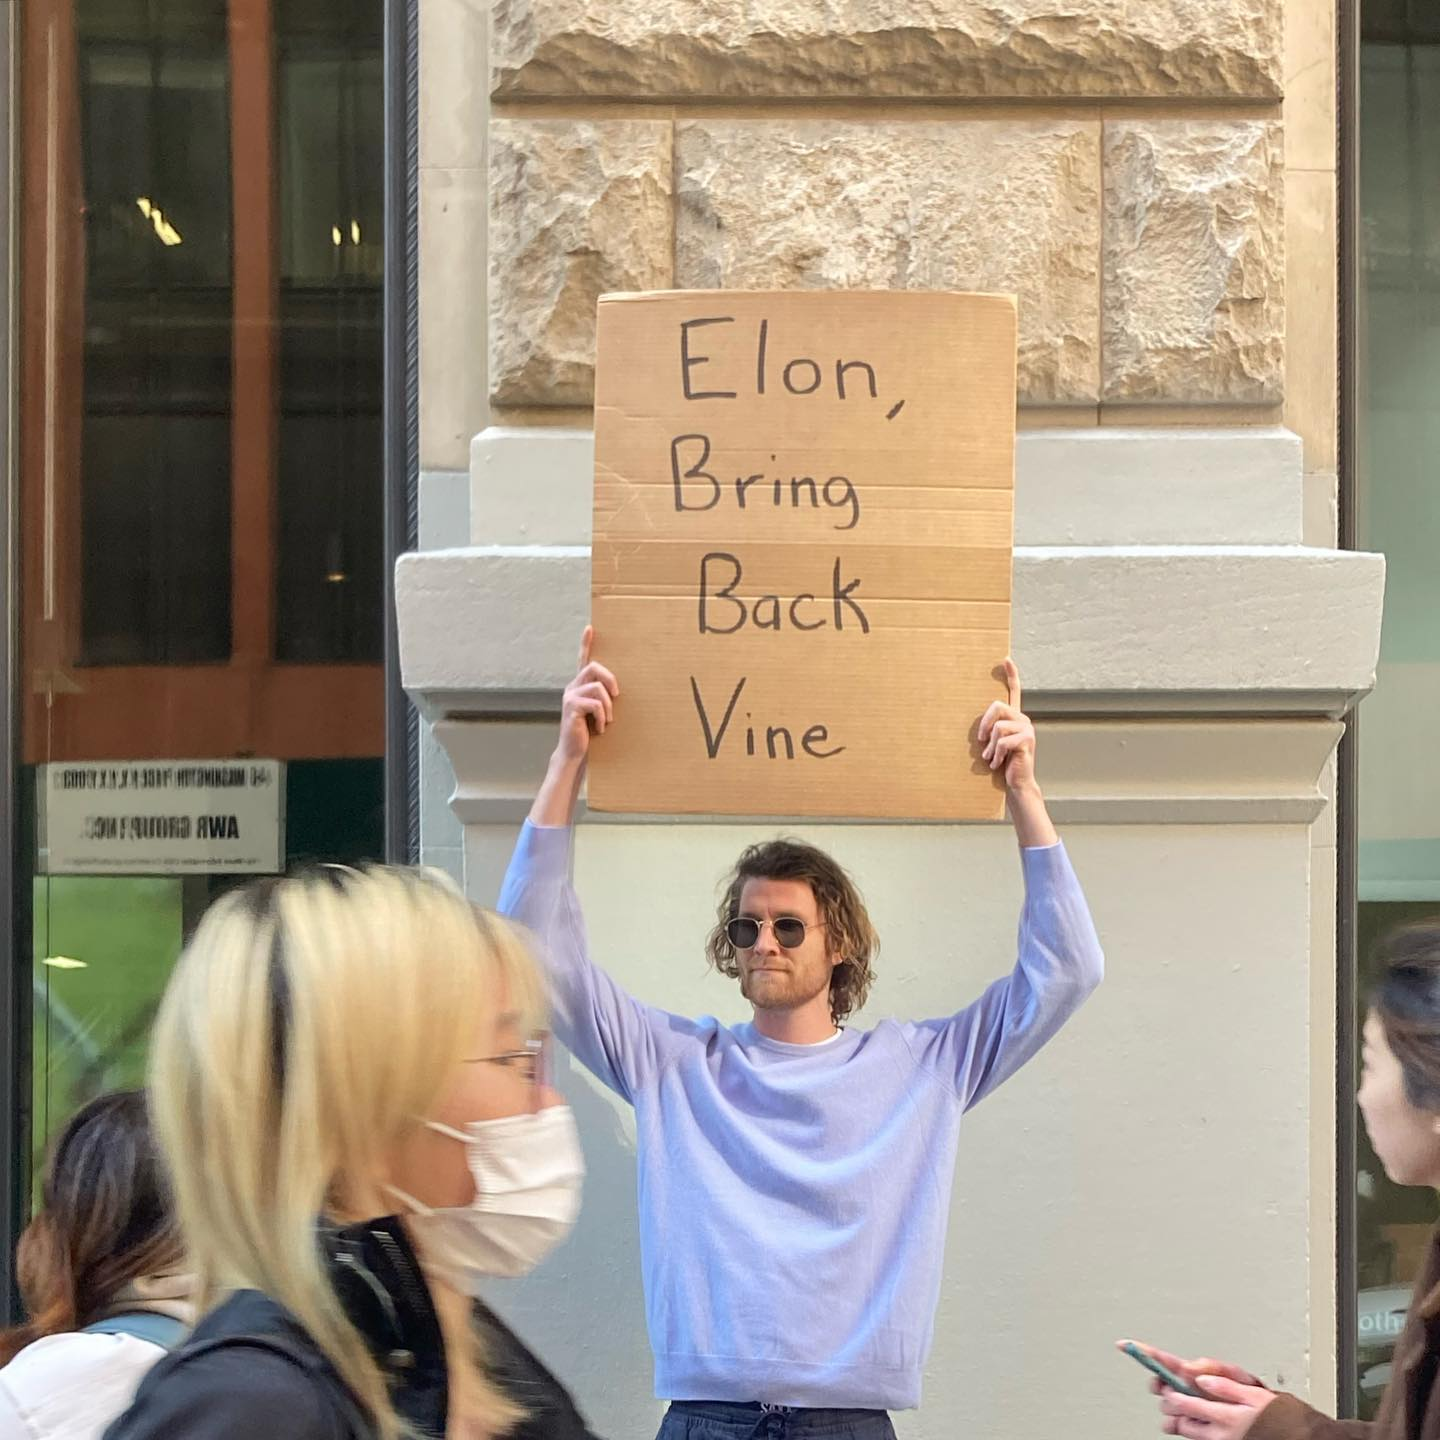
\includegraphics{img/dudewithsign.jpeg}}\end{minipage}%
%
\begin{minipage}{0.02\linewidth}
~\end{minipage}%
%
\begin{minipage}{0.49\linewidth}
\href{https://fitchburgstate.edu}{Fitchburg State University}\\
\href{https://www.fitchburgstate.edu/academics/academic-schools/school-arts-and-sciences/communications-media-department}{Communications
Media Department}\\
\href{https://www.fitchburgstate.edu/academics/programs/social-media-concentration-applied-communication-ms-online}{MS
in Applied Communication: Social Media Concentration}\\
GCE Online-Accelerated\\
7 weeks, Tues 29 October---Tues 17 December 2024\\
Instructor: Martin Roberts\\
\href{https://mroberts1.github.io/fsu-smt-su24}{Syllabus}\\
\href{mailto:mrober40@fitchburgstate.edu}{\faIcon{envelope}} \textbar{}
\href{https://github.com/mroberts1/fsu-social-mobilities-fa24}{\faIcon{github}}
\textbar{} \href{https://discord.gg/GUSz99EP}{\faIcon{discord}}
\textbar{}
\href{https://www.youtube.com/playlist?list=PLx7AcHafElRiGpYPLRM29YzNMMEXyDqmh}{\faIcon{youtube}}\end{minipage}%

\end{figure}%

\subsection{Overview}\label{overview}

This seminar is an exploration of what it means to live with personal,
portable, and handheld media technologies. We will study these
technologies across time and space by situating them within their
historical contexts and by studying their use in various settings. We'll
also employ a variety of theoretical frameworks and interdisciplinary
approaches. Simultaneously, we will attempt to analyze and theorize our
own handheld media experiences through and against the course readings.

\subsection{Objectives}\label{objectives}

By the end of the course, students will be able to:

\begin{itemize}
\tightlist
\item
  analyze technologies past, present, and imagined
\item
  describe the ways in which technologies shape our world the ways in
  which we shape those technologies
\item
  explain how social media is a result of the intersection between
  technologies and existing human communication dynamics
\item
  discuss how theory of technology and social media can improve the
  vocational outlook of a student
\item
  play a productive role in and facilitate conversations that tease out
  the relationships between values and technology.
\item
  through the skills you will refine in writing your research papers,
  clearly explain how a specific technology shapes the social world that
  we live in.
\end{itemize}

\subsection{Course Texts}\label{course-texts}

Available as audiobooks (Audible) and ebooks (Kindle), as well as print.

\href{https://www.kylechayka.com/}{Kyle Chayka}, \textbf{Filterworld:
How Algorithms Flattened Culture}. New York: Doubleday, 2024.

\href{https://emerson.edu/faculty-staff-directory/kate-eichhorn}{Kate
Eichhorn},
\href{https://mitpress.mit.edu/9780262543286/content/}{\textbf{Content}}.
Essential Knowledge Series. Cambridge, MA: MIT Press, 2022.

\href{https://x.com/parmy}{Parmy Olson}, \textbf{Supremacy: AI, ChatGPT,
and the Race that Will Change the World}. New York: MacMillan, 2024.

\href{https://x.com/lagorio}{Christine Lagorio-Chafkin}, \textbf{We Are
the Nerds: The Birth and Tumultuous Life of Reddit, the Internet's
Culture Laboratory}. New York: Hachette Books, 2018.

\href{https://allissavrichardson.com}{Allissa V. Richardson},
\textbf{Bearing Witness While Black: African Americans, Smartphones, and
the New Protest \#Journalism}. Oxford: Oxford University Press, 2020.

Stefania Maurizi, \textbf{Secret Power: Wikileaks and Its Enemies}.
Pluto Press, 2023.

\begin{center}\rule{0.5\linewidth}{0.5pt}\end{center}

\subsubsection{Documentaries}\label{documentaries}

\textbf{Citizenfour} (2014)\\
\textbf{Risk} (2016)\\
\textbf{Super Pumped: The Battle for Uber} (Showtime, 2022)\\
\textbf{We Are Legion: The Story of the Hacktivists} (2012)\\
\textbf{WeWork: Or the Making and Breaking of a \$47 Billion Unicorn}
(Hulu, 2021)\\
\textbf{Wikileaks: Secrets and Lies} (2011)\\

\begin{center}\rule{0.5\linewidth}{0.5pt}\end{center}

\subsection{Course Information}\label{course-information}

\textbf{Platforms}\\
We'll be using Blackboard for submitting assignments ONLY. For
discussion, we will be using
\href{https://discord.gg/GUSz99EP}{Discord}.

On Discord, if you don't already have an account, please set one up
using your Fitchburg State University email address as ID.

If you already have a Discord account there will be problems setting up
an account for the course because each account has to be tied to a
different phone number, so you will not be able to use your regular
phone number for verification. For this reason, you may use your
existing account, but if you use a pseudonym please let me know what
this is so I know who you are!

Please be sure to check in to the site at least once daily M-F to check
the Announcements page and the Discussion forum for the week.

\begin{center}\rule{0.5\linewidth}{0.5pt}\end{center}

\subsection{Assignments \& Evaluation}\label{assignments-evaluation}

\textbf{Review}\\
6, weekly from Week 1, one short post responding to readings, 250 words
(maximum), due by Sunday of each week (20\%)

\textbf{Discord}\\
Regular participation in weekly discussion and other channels (20\%)

\textbf{Commentary papers}\\
2 short analysis papers (500 words, 2 pages double-spaced) based on any
of the reading assignments, due on Blackboard by end of Weeks 2 and 4
(Sunday) (20\%)

\textbf{Book Report}\\
Critical review (1,000 words, 4 pages double-spaced) of any text from
the select bibliography. You are expected to read at least one
additional chapter from any of the main course books. For texts
scheduled in weeks 5-6, you'll need to read ahead. Due on Blackboard by
Friday of Week 5 (20\%)

\textbf{Research paper/report/creative project}~ 2,000 words, due on
Blackboard by Friday of Week 7 (20\%)

The culminating written assignment for the course (2,000 words) may
consist of various formats: a research paper or report, or a creative
project (blog, website, podcast)

A 1-page tentative proposal with ideas for your project, with a short
bibliography with sources and/or links, should be posted in the
Discussion forum on Blackboard by the end of Week 4, and you will
receive feedback during Week 5.

\begin{center}\rule{0.5\linewidth}{0.5pt}\end{center}

By \textbf{Wednesday} of each week, I will post an Agenda item in the
Discussion forum for the topic of the week, that introduces and
contextualizes the reading assignments for the week, identifying key
themes, concepts, and/or issues to look out for as you read.

\textbf{Commentary Papers}\\
These short papers (750-1,000 words) are due at the end of Week 2 and
Week 4 (Sunday). They should consist of analytical close readings of any
of the reading assignments for the period Weeks 1-2 or 3-4. You are
encouraged to focus in detail on particular sections, arguments, and/or
concepts from the readings and develop them.

\textbf{Research Paper/Project}\\
The culminating written assignment for the course (2,000 words) may
consist of various formats: a research paper or report, or a creative
project of your choice.

A 1-page preliminary proposal with ideas for your project, with a short
bibliography with sources and/or links, should be posted in the
Discussion forum for the purpose by the end of Week 3, and you will
receive feedback during Week 4.

\begin{center}\rule{0.5\linewidth}{0.5pt}\end{center}

\subsection{Schedule}\label{schedule}

Week 1: Tuesday 29 October 2024

\textbf{Content}

\href{https://emerson.edu/faculty-staff-directory/kate-eichhorn}{Kate
Eichhorn}, \textbf{Content}:

\begin{itemize}
\tightlist
\item
  ``\href{pdf/eichhorn-content-ch1.pdf}{A Brief History of Content in a
  Digital Era}''
\item
  ``\href{pdf/eichhorn-content-ch2.pdf}{User-Generated Content}''
  (recommended)
\end{itemize}

See also: Patrick H. Willems,
``\href{https://youtu.be/hAtbFwzZp6Y}{Everything is Content Now}''
(YouTube)

\begin{center}\rule{0.5\linewidth}{0.5pt}\end{center}

Week 2: Tuesday 5 November 2024

\textbf{Algorithm}

\href{https://www.kylechayka.com/}{Kyle Chayka}, \textbf{Filterworld:
How Algorithms Flattened Culture}

\begin{itemize}
\tightlist
\item
  ``\href{pdf/filterworld-intro.pdf}{Introduction}''
\item
  ``\href{pdf/filterworld-ch1.pdf}{The Rise of Algorithmic
  Recommendations}'' (ch.~1)
\end{itemize}

\begin{center}\rule{0.5\linewidth}{0.5pt}\end{center}

Week 3: Tuesday 12 November 2024

\textbf{Chatbot}

\href{https://x.com/parmy}{Parmy Olson}, \textbf{Supremacy: How the
Struggle Between Google and Facebook Shapes Our Future}

\begin{itemize}
\tightlist
\item
  ``\href{pdf/supremacy-prologue.pdf}{Prologue}''
\item
  ``\href{pdf/supremacy-ch12.pdf}{Mythbusters}'' (ch.~12)
\item
  ``\href{pdf/supremacy-ch13.pdf}{Hello, ChatGPT}'' (ch.~13)
\end{itemize}

\begin{center}\rule{0.5\linewidth}{0.5pt}\end{center}

Week 4: Tuesday 19 November 2024

\textbf{Nerd}

\href{https://x.com/lagorio}{Christine Lagorio-Chafkin}, \textbf{We Are
the Nerds: The Birth and Tumultuous Life of Reddit, the Internet's
Culture Laboratory}

\begin{itemize}
\tightlist
\item
  \href{pdf/lagorio-wearethenerds-part1.pdf}{\emph{We Are the Nerds},
  part I}
\end{itemize}

\begin{center}\rule{0.5\linewidth}{0.5pt}\end{center}

Week 5: Tuesday 26 November 2024

\textbf{Witness}

Allissa V. Richardson, \textbf{Bearing Witness While Black}

\begin{center}\rule{0.5\linewidth}{0.5pt}\end{center}

Week 6: Tuesday 3 December 2024

\textbf{Whistleblower}

Stefania Maurizi, \textbf{Secret Power: Wikileaks and Its Enemies}

\begin{center}\rule{0.5\linewidth}{0.5pt}\end{center}

Week 7: Tuesday 10 December 2024

Research projects

Tuesday 17 December 2024: Last day of classes

\begin{center}\rule{0.5\linewidth}{0.5pt}\end{center}

\subsection{Bibliography}\label{bibliography}

danah boyd, \textbf{It's Complicated: The Social Lives of Networked
Teens} (New Haven: Yale University Press, 2014).

Amy Bruckman, \textbf{Should You Believe Wikipedia? Online Communities
and the Construction of Knowledge} (Cambridge: Cambridge University
Press, 2022).

Finn Brunton and Helen Nissenbaum, \textbf{Obfuscation: A User's Guide
for Privacy and Protest} (Cambridge: MIT Press, 2016).

Kyle Chayka, \textbf{Filterworld: How Algorithms Flattened Culture} (New
York: Doubleday, 2024).

Gabriella Coleman, \textbf{Hacker, Hoaxer, Whistleblower, Spy: The Many
Faces of Anonymous} (London and New York: Verso, 2014).

Claire Dederer, \textbf{Monsters: A Fan's Dilemma} (New York: Alfred A.
Knopf, 2023).

\href{https://emerson.edu/faculty-staff-directory/kate-eichhorn}{Kate
Eichhorn},
\href{https://mitpress.mit.edu/9780262543286/content/}{\textbf{Content}}.
Essential Knowledge Series (Cambridge, MA: MIT Press, 2022).

Glenn Greenwald, \textbf{No Place to Hide: Edward Snowden, the NSA, and
the U.S. Surveillance State} (New York: Metropolitan Books, 2014).

Adrian Hon, \textbf{You've Been Played: How Corporations, Governments,
and Schools Use Games to Control Us All} (New York: Basic Books, 2022).

Sarah J. Jackson, Moya Bailey, et al., \textbf{\#Hashtag Activism:
Networks of Race and Gender Justice} (Cambridge: MIT Press, 2020).

\href{https://x.com/lagorio}{Christine Lagorio-Chafkin}, \textbf{We Are
the Nerds: The Birth and Tumultuous Life of Reddit, the Internet's
Culture Laboratory} (New York: Hachette Books, 2018).

Taylor Lorenz, \textbf{Extremely Online: How the Internet Changed the
Way We Live, Love, Work, and Play} (New York: Simon \& Schuster, 2022\}.

Gary Marcus \& Ernest Davis, \textbf{Rebooting AI: Building Artificial
Intelligence We Can Trust} (New York: Pantheon Books, 2019).

Stefania Maurizi, \textbf{Secret Power: Wikileaks and Its Enemies}.
Pluto Press, 2023.

\href{https://gretchenmcculloch.com/}{Gretchen McCulloch},
\href{https://gretchenmcculloch.com/book/}{\textbf{Because Internet:
Understanding the New Rules of Language}} (Riverhead Books, 2019)

Angela Nagle, \textbf{Kill All Normies: Online Culture Wars From 4Chan
and Tumblr to Trump and the Alt-Right} (Alresford, Hampshire, UK: Zero
Books, 2017).

\href{https://x.com/parmy}{Parmy Olson}, \textbf{Supremacy: AI, ChatGPT,
and the Race that Will Change the World}. New York: MacMillan, 2024.

Cathy O'Neil, with Stephen Baker, \textbf{The Shame Machine: Who Profits
in the New Age of Humiliation} (New York: Crown/Random House, 2022).

Whitney Phillips, \textbf{This Is Why We Can't Have Nice Things: Mapping
the Relationship between Online Trolling and Mainstream Culture}
(Cambridge: MIT Press, 2015).

Whitney Phillips and Ryan M. Milner, \textbf{You Are Here: A Field Guide
for Navigating Polarized Speech, Conspiracy Theories, and Our Polluted
Media Landscape} (Cambridge: MIT Press, 2021).

Allissa V, Richardson, \textbf{Bearing Witness While Black: African
Americans, Smartphones, and the New Protest \#Journalism} (Oxford:
Oxford University Press, 2020).

Zeynep Tufekci, \textbf{Twitter and Tear Gas: The Power and Fragility of
Networked Protes} (New Haven: Yale University Press, 2017\}.

Michele White, \textbf{Touch Screen Theory: Digital Devices and
Feelings} (Cambridge, MA: MIT Press, 2022).

Christopher Wylie, \textbf{Mindf**k: Cambridge Analytica and the Plot to
Break America} (New York: Random House, 2019).

\begin{center}\rule{0.5\linewidth}{0.5pt}\end{center}

\subsection{Policies}\label{policies}

\textbf{Late Policy}

Assignments that are late will lose 1/2 of a grade per day, beginning at
the end of class and including weekends and holidays. This means that a
paper, which would have received an A if it was on time, will receive a
B+ the next day, B- for two days late, and so on. Time management,
preparation for our meetings, and timely submission of your work
comprise a significant dimension of your professionalism. As such, your
work must be completed by the beginning of class on the day it is due.
If you have a serious problem that makes punctual submission impossible,
you must discuss this matter with me before the due date so that we can
make alternative arrangements. Because you are given plenty of time to
complete your work, and major due dates are given to you well in
advance, last minute problems should not preclude handing in assignments
on time.

\textbf{Mandatory Reporter}

Fitchburg State University is committed to providing a safe learning
environment for all students that is free of all forms of discrimination
and harassment. Please be aware all FSU faculty members are ``mandatory
reporters,'' which means that if you tell me about a situation involving
sexual harassment, sexual assault, dating violence, domestic violence,
or stalking, I am legally required to share that information with the
Title IX Coordinator. If you or someone you know has been impacted by
sexual harassment, sexual assault, dating or domestic violence, or
stalking, FSU has staff members trained to support you. If you or
someone you know has been impacted by sexual harassment, sexual assault,
dating or domestic violence, or stalking, please visit
\url{http://fitchburgstate.edu/titleix} to access information about
university support and resources.

\textbf{Health}

\href{http://www.google.com/url?q=http\%3A\%2F\%2Fwww.fitchburgstate.edu\%2Foffices-services-directory\%2Fhealth-services\%2F&sa=D&sntz=1&usg=AFQjCNEw5V0i0hL5DVO5b43gejNNaAt4ig}{Health
Services}

Hours: Monday-Friday 8:30AM-5PM Location: Ground Level of Russell Towers
(across from the entrance of Holmes Dining Hall) Phone: (978)
665-3643/3894

\href{http://www.google.com/url?q=http\%3A\%2F\%2Fwww.fitchburgstate.edu\%2Foffices-services-directory\%2Fcounseling-services\%2F&sa=D&sntz=1&usg=AFQjCNEYiS4EmSvWerpp2bKr5lTpouPuqQ}{Counseling
Services}

The Counseling Services Office offers a range of services including
individual, couples and group counseling, crisis intervention,
psychoeducational programming, outreach ALTERNATIVE ECOSYSTEMSs, and
community referrals. Counseling services are confidential and are
offered at no charge to all enrolled students. Staff at Counseling
Services are also available for consultation to faculty, staff and
students. Counseling Services is located in the Hammond, 3rd Floor, Room
317.

\href{http://www.google.com/url?q=http\%3A\%2F\%2Fwww.fitchburgstate.edu\%2Foffices-services-directory\%2Ffitchburg-anti-violence-education\%2F&sa=D&sntz=1&usg=AFQjCNFi5qy-wunMxX-hoWbA9YwT8aa4Ig}{Fitchburg
Anti-Violence Education (FAVE)}

FAVE collaborates with a number of community partners (e.g., YWCA
Domestic Violence Services, Pathways for Change) to meet our training
needs and to link survivors with community based resources. This site
also features
\href{http://www.google.com/url?q=http\%3A\%2F\%2Fwww.fitchburgstate.edu\%2Foffices-services-directory\%2Ffitchburg-anti-violence-education\%2Ffitchburg-anti-violence-education-resources\%2F&sa=D&sntz=1&usg=AFQjCNF9KZ2O1AvPMLJTHdNg1DfmYYtgog}{resources}
for help or information about dating violence, domestic violence, sexual
assault and stalking. If you or someone you know is in an abusive
relationship or has been a victim of sexual assault, there are many
places to go for help. Many can be accessed 24 hours a day, seven days a
week, 365 days a year. On campus, free and confidential support is
provided at both Counseling Services and Health Services.

\emph{Community Food Pantry} Food insecurity is a growing issue and it
certainly can affect student learning. The ability to have access to
nutritious food is incredibly vital. The Falcon Bazaar, located in
Hammond G 15, is stocked with food, basic necessities, and can provide
meal swipes to support all Fitchburg State students experiencing food
insecurity for a day or a semester.

The university continues to partner with Our Father's House to support
student needs and access to food and services. All Fitchburg State
University students are welcome at the Our Father's House Community Food
Pantry. This Pantry is located at the Faith Christian Church at 40
Boutelle St., Fitchburg, MA and is open from 5-7pm. Each ``household''
may shop for nutritious food once per month by presenting a valid FSU
ID.

\textbf{Academic Integrity}

The University ``Academic Integrity'' policy can be found online at
\href{http://www.fitchburgstate.edu/offices-services-directory/office-of-student-conduct-mediation-education/academic-integrity/}{http://
www.fitchburgstate.edu/offices-services-directory/office-of-student-conductmediation-education/academic-integrity/.}
Students are expected to do their own work. Plagiarism and cheating are
inexcusable. Any instance of plagiarism or cheating will automatically
result in a zero on the assignment and may be reported the Office of
Student and Academic Life at the discretion of the instructor.

Plagiarism includes, but is not limited to: - Using papers or work from
another class. - Using another student's paper or work from any class. -
Copying work or a paper from the Internet. - The egregious lack of
citing sources or documenting research.

\emph{If you're not clear on what is or is not plagiarism, ASK. The BEST
case scenario if caught is a zero on that assignment, and ignorance of
what does or does not count is not an excuse. That being said, I'm a
strong supporter of}
\href{https://en.wikipedia.org/wiki/Fair_Use}{\emph{Fair Use}}
\emph{doctrine. Just attribute what you use--and, again, ASK if there's
any doubt.}

\textbf{Americans With Disabilities Act (ADA)}

If you need course adaptations or accommodations because of a
disability, if you have emergency medical information to share with the
instructor, or if you need special arrangements in case the building
must be evacuated, please inform the faculty member as soon as possible.

\textbf{Technology}

At some point during the semester you will likely have a problem with
technology. Your laptop will crash; your iPad battery will die; a
recording you make will disappear; you will accidentally delete a file;
the wireless will go down at a crucial time. These, however, are
inevitabilities of life, not emergences. Technology problems are not
excuses for unfinished or late work. Bad things may happen, but you can
protect yourself by doing the following:

\begin{itemize}
\item
  Plan ahead: A deadline is the last minute to turn in material. You can
  start---and finish---early, particularly if challenging resources are
  required, or you know it will be time consuming to finish this
  project.
\item
  Save work early and often: Think how much work you do in 10 minutes. I
  auto save every 2 minutes.
\item
  Make regular backups of files in a different location: Between Box,
  Google Drive, Dropbox, and iCloud, you have ample places to store and
  backup your materials. Use them.
\item
  Save drafts: When editing, set aside the original and work with a
  copy.
\item
  Practice safe computing: On your personal devices, install and use
  software to control viruses and malware.
\end{itemize}

\textbf{Grading Policy}

Grading for the course will follow the FSU grading policy below:

4.0: 95-100\\
3.7: 92-94\\
3.5: 89-91\\
3.3: 86-88\\
3.0: 83-85\\
2.7: 80-82\\
2.5: 77-79\\
2.3: 74-76\\
2.0: 71-73\\
0.0: \textless{} 70

\textbf{Academic Resources}

\href{http://www.fitchburgstate.edu/offices-services-directory/tutor-center/writing-help/}{Writing
Center}

\href{http://catalog.fitchburgstate.edu/content.php?catoid=13&navoid=851}{Academic
Policies}

\href{http://www.fitchburgstate.edu/offices-services-directory/disability-services/}{Disability
Services}

\href{https://www.getrave.com/login/fitchburgstate/}{Fitchburg State
Alert system for emergencies, snow closures/delays, and faculty
absences}

\href{http://www.fitchburgstate.edu/offices-services-directory/career-counseling-and-advising/careerservices/}{University
Career Services}




\end{document}
